\section{Experimental Setup and Methodology}
\label{sec:methodology}

\begin{table*}[!t]
\centering
\caption{Experimental Hardware, Software Testbeds, and Benchmarking Workload Parameters}
\label{tab:environment}
\scriptsize
\renewcommand{\arraystretch}{0.93}
\begin{tabular*}{\textwidth}{@{\extracolsep{\fill}}lll}
\toprule
\textbf{Parameter / Dimension} & \textbf{Primary Testbed (Fedora 45)} & \textbf{Comparative Testbed (WSL2)} \\
\midrule
\textbf{Host Architecture} & Intel(R) Core(TM) 7 240H (x86\_64) & AMD Ryzen 7 8845HS (x86\_64) \\
\textbf{Core Topology} & 4 Dedicated VCPUs (Host: 16) & 16 Virtual Processors \\
\textbf{Operating System} & Fedora 45 Linux & Ubuntu 26.04 LTS (WSL2) \\
\textbf{Kernel Release} & \texttt{7.3.3-300.fc45.x86\_64} & \texttt{6.6.87.2-microsoft-standard} \\
\textbf{Memory Capacity} & 3.8 GiB DDR5 & 15.3 GiB DDR5 \\
\textbf{C Compiler} & GCC 16.2.1 20261029 (Red Hat) & GCC 13.3.0 (Ubuntu) \\
\textbf{Compiler Flags} & \multicolumn{2}{l}{\texttt{-std=c11 -O2 -Wall -Wextra -D\_GNU\_SOURCE}} \\
\textbf{CPU Core Affinity} & Core 0 (Producer) / Core 1 (Consumer) & Core 0 (Producer) / Core 1 (Consumer) \\
\midrule
\textbf{Payload Sweep} & \multicolumn{2}{l}{64 B, 256 B, 1024 B, 4096 B, 16384 B, 65536 B, 262144 B} \\
\textbf{Measurement Loop} & \multicolumn{2}{l}{10,000 timed round-trip exchanges per trial} \\
\textbf{Untimed Warm-up} & \multicolumn{2}{l}{500 untimed exchanges preceding measurement} \\
\textbf{Independent Trials} & \multicolumn{2}{l}{$N = 7$ randomized trial blocks per configuration cell} \\
\textbf{Sampling Method} & \multicolumn{2}{l}{\texttt{clock\_gettime(CLOCK\_MONOTONIC)} (Nanosecond resolution)} \\
\textbf{Percentile Metric} & \multicolumn{2}{l}{Nearest-rank method ($P_{50}, P_{90}, P_{95}, P_{99}, P_{99.9}$)} \\
\bottomrule
\end{tabular*}
\end{table*}


Rigorous performance evaluation of low-level systems software requires strict environmental isolation, reproducible execution protocols, and verifiable statistical metrics~\cite{gregg2020systems}. This section details our experimental testbed, workload configurations, and profiling methodology. Fig.~\ref{fig:benchmark_workflow} illustrates the end-to-end benchmark workflow.

\begin{figure*}[!t]
\centering
\begin{tikzpicture}[
    scale=0.82, every node/.style={transform shape},
    box/.style={draw=darknavy, rounded corners=3pt, text width=3.35cm, minimum height=0.82cm, align=center},
    stageI/.style={box, fill=acadblue!15, draw=acadblue, thick},
    ctrlI/.style={box, fill=mutedorange!18, draw=mutedorange, thick},
    statII/.style={box, fill=mutedgreen!18, draw=mutedgreen, thick},
    outII/.style={box, fill=darknavy!15, draw=darknavy, thick},
    arr/.style={->, >=stealth, very thick, draw=charcoal}
]

% Row 1: Stage I - Execution & Scientific Controls (Left to Right)
\node[stageI] (n1) at (0.0, 1.55) {
    \textbf{\scriptsize 1. Workload Sweep}\\[1pt]
    \tiny 64 B to 256 KB Sweep\\
    \tiny 10,000 Exchanges / Trial
};

\node[ctrlI] (n2) at (4.2, 1.55) {
    \textbf{\scriptsize 2. Scientific Controls}\\[1pt]
    \tiny Fisher-Yates Shuffling\\
    \tiny Dedicated CPU Pinning
};

\node[ctrlI] (n3) at (8.4, 1.55) {
    \textbf{\scriptsize 3. Untimed Warm-Up}\\[1pt]
    \tiny 500 Untimed Cycles\\
    \tiny Cache \& TLB Priming
};

\node[stageI] (n4) at (12.6, 1.55) {
    \textbf{\scriptsize 4. Precision Hot Loop}\\[1pt]
    \tiny \texttt{CLOCK\_MONOTONIC}\\
    \tiny Low-ns vDSO Monotonic Timer
};

% Row 2: Stage II - Analysis & Verification (Right to Left)
\node[statII] (n5) at (12.6, 0.0) {
    \textbf{\scriptsize 5. Statistical Engine}\\[1pt]
    \tiny Nearest-Rank $P_{50}$--$P_{99.9}$\\
    \tiny Mean, Stdev, Wire Bandwidth
};

\node[statII] (n6) at (8.4, 0.0) {
    \textbf{\scriptsize 6. OS Resource Telemetry}\\[1pt]
    \tiny \texttt{getrusage} Context Switches\\
    \tiny User/Sys CPU, Peak RSS
};

\node[statII] (n7) at (4.2, 0.0) {
    \textbf{\scriptsize 7. Adaptive Telemetry}\\[1pt]
    \tiny Empirical Oracle Regret\\
    \tiny EWMA ($\alpha=0.15$) \& Hysteresis
};

\node[outII] (n8) at (0.0, 0.0) {
    \textbf{\scriptsize 8. Research Artifacts}\\[1pt]
    \tiny 13 Vector Visualizations\\
    \tiny Verified LaTeX Tables
};

% Background Groups with clean banners
\begin{scope}[on background layer]
    \node[draw=acadblue!50, dashed, fill=acadblue!4, rounded corners=4pt, fit=(n1) (n4), inner ysep=5pt, inner xsep=4pt,
          label={[font=\scriptsize\bfseries, text=acadblue]above:STAGE I: BENCHMARK EXECUTION AND SCIENTIFIC CONTROLS}] {};
    \node[draw=mutedgreen!60, dashed, fill=mutedgreen!4, rounded corners=4pt, fit=(n8) (n5), inner ysep=5pt, inner xsep=4pt,
          label={[font=\scriptsize\bfseries, text=mutedgreen!80!black]below:STAGE II: STATISTICAL ANALYSIS AND TELEMETRY EXTRACTION}] {};
\end{scope}

% Forward Arrows
\draw[arr] (n1) -- (n2);
\draw[arr] (n2) -- (n3);
\draw[arr] (n3) -- (n4);
\draw[arr] (n4) -- (n5);
\draw[arr] (n5) -- (n6);
\draw[arr] (n6) -- (n7);
\draw[arr] (n7) -- (n8);

\end{tikzpicture}

\caption{End-to-End Unified Experimental Benchmarking Workflow, detailing trial-block randomization, CPU pinning, cache warm-up, and metrics extraction.}
\label{fig:benchmark_workflow}
\end{figure*}

\subsection{Hardware and Software Environment}
All primary experimental evaluations were conducted within a dedicated, isolated Linux systems environment. Table~\ref{tab:environment} lists the detailed system specifications and benchmark workload parameters.

The primary experimental testbed runs Fedora 45 Linux within a Kernel-based Virtual Machine (KVM) guest environment, powered by an Intel(R) Core(TM) 7 240H host processor (x86\_64) with 4 dedicated virtual CPUs (vCPUs) and 3.8~GiB of DDR5 memory. The operating system runs Linux kernel \texttt{7.3.4-300.fc45.x86\_64} configured with dynamic preemption (\texttt{PREEMPT\_DYNAMIC}). All benchmarks and test harnesses were compiled natively using GCC 16.2.1 20261029 with optimization flags \texttt{-std=c11 -O2 -Wall -Wextra -D\_GNU\_SOURCE}. This environment provides uninhibited access to modern Linux kernel subsystems, complete POSIX compliance, preemptible scheduling, and native System V IPC facilities.

\subsection{Workload Configurations and Scientific Controls}
The benchmarking matrix evaluates seven discrete payload sizes spanning four orders of magnitude: $\mathcal{S} = \{64\text{ B}, 256\text{ B}, 1\text{ KB}, 4\text{ KB}, 16\text{ KB}, 64\text{ KB}, 256\text{ KB}\}$.
For each payload size and mechanism, the benchmark executes $N = 7$ independent trial blocks. Each trial consists of 10,000 timed round-trip ping-pong exchanges preceded by 500 untimed warm-up exchanges, yielding 70,000 recorded exchanges per configuration cell. Across all 7 mechanism modes and 7 payload classes evaluated over 7 trial blocks, the test harness scheduled 3,430,000 single-pair exchanges ($7 \times 7 \times 7 \times 10,000$), recording 2,730,000 valid timed round-trip ping-pong exchanges across supported configurations (along with 171,500 untimed warm-up cycles, 525,000 concurrent pipeline messages, 140,000 mixed-payload exchanges, and 150,000 streaming transfers, totaling over 3.71 million experimental exchanges and exceeding 4.5 million discrete message transfers).

To eliminate confounding measurement artifacts, the benchmarking harness enforces four scientific controls:
\begin{enumerate}[leftmargin=*,noitemsep,topsep=1.5pt]
    \item \textbf{Untimed Cache and TLB Priming:} Executing 500 untimed exchanges before measurement ensures that virtual memory pages are faulted in, CPU translation lookaside buffers (TLB) are populated, and kernel data structures reside in L1/L2 caches.
    \item \textbf{Trial-Block Randomization:} Mechanism execution order within each trial block is shuffled using a deterministic Fisher-Yates generator. This prevents thermal throttling or periodic operating system background daemons from systematically biasing a specific transport.
    \item \textbf{Strict CPU Affinity Pinning:} Processes are bound to guest virtual CPU cores (vCPU~0 for the producer and vCPU~1 for the consumer) via \texttt{sched\_setaffinity}. This isolates execution pipelines across virtual processors, while underlying physical core dispatch remains managed by the host hypervisor scheduler.
    \item \textbf{High-Resolution Timing:} Timing measurements utilize \texttt{clock\_gettime(CLOCK\_MONOTONIC)}, which is served through the Linux virtual dynamic shared object (vDSO) on supported configurations to minimize system-call boundary crossings, with low nanosecond measurement overhead depending on the host timer source and hypervisor clock virtualization.
\end{enumerate}

\subsection{Performance Metrics}
We report comprehensive latency, throughput, and system resource metrics:
\begin{itemize}[leftmargin=*,noitemsep,topsep=1.5pt]
    \item \textbf{Mean Round-Trip Latency ($\mu\text{s}$):} Arithmetic mean of round-trip transfer times across all measured iterations: $\bar{L} = \frac{1}{K} \sum_{i=1}^K (t_{\text{recv}, i} - t_{\text{send}, i})$ where $K = 10,000$ iterations.
    \item \textbf{Tail Latency Percentiles ($P_{50}, P_{90}, P_{95}, P_{99}$):} Computed using the integer nearest-rank method over sorted sample arrays: $k = \lceil \frac{p}{100} \cdot K \rceil - 1$.
    \item \textbf{Throughput (msg/s and MB/s):} Message frequency and wire bandwidth: $\text{Throughput}_{\text{msg/s}} = K / \Delta t_{\text{total}}$ and $\text{Throughput}_{\text{MB/s}} = (K \cdot s) / (1024^2 \cdot \Delta t_{\text{total}})$.
    \item \textbf{Operating System Telemetry:} Gathered via \texttt{getrusage} (\texttt{RUSAGE\_SELF} and \texttt{RUSAGE\_CHILDREN}), capturing voluntary and involuntary context switches, CPU time, and peak RSS. System calls are classified via Linux \texttt{strace}.
\end{itemize}

% Queue Table III and Figure 5 for the top of Section VII on Page 8
\begin{table*}[t]
\centering
\caption{Mean Round-Trip Latency ($\mu\text{s}$) Across Payload Sizes on Fedora 45 Linux ($N=7$ Trials, 10,000 Exchanges/Trial)}
\label{tab:benchmark_results}
\scriptsize
\begin{tabular}{lrrrrrrr}
\toprule
\textbf{Mechanism} & \textbf{64 B} & \textbf{256 B} & \textbf{1,024 B} & \textbf{4,096 B} & \textbf{16,384 B} & \textbf{65,536 B} & \textbf{262,144 B} \\
\midrule
\textbf{Anonymous Pipe} & 399.25 $\pm$ 23.1 & 344.57 $\pm$ 19.8 & \textbf{278.76} $\pm$ 14.5 & \textbf{301.70} $\pm$ 16.2 & \textbf{472.79} $\pm$ 22.4 & \textbf{505.93} $\pm$ 24.1 & 4,548.77 $\pm$ 180.2 \\
\textbf{Named FIFO} & 464.27 $\pm$ 28.4 & 456.39 $\pm$ 25.1 & 619.56 $\pm$ 34.2 & 454.10 $\pm$ 26.8 & 584.14 $\pm$ 31.0 & 633.72 $\pm$ 35.4 & 4,217.02 $\pm$ 172.5 \\
\textbf{System V MQ} & 359.59 $\pm$ 21.0 & 395.60 $\pm$ 22.5 & 317.58 $\pm$ 18.2 & 331.48 $\pm$ 19.4 & \textit{Limit} & \textit{Limit} & \textit{Limit} \\
\textbf{POSIX MQ} & 499.72 $\pm$ 29.5 & 767.24 $\pm$ 48.2 & 477.91 $\pm$ 27.6 & 534.33 $\pm$ 30.1 & \textit{Limit} & \textit{Limit} & \textit{Limit} \\
\textbf{POSIX SHM} & \textbf{286.87} $\pm$ 12.4 & \textbf{320.35} $\pm$ 15.6 & 351.15 $\pm$ 17.8 & \textit{Limit} & \textit{Limit} & \textit{Limit} & \textit{Limit} \\
\textbf{Unix Domain Skt} & 618.33 $\pm$ 35.2 & 619.67 $\pm$ 34.8 & 674.68 $\pm$ 39.1 & 720.01 $\pm$ 41.5 & 571.35 $\pm$ 32.7 & 648.34 $\pm$ 38.2 & \textbf{2,590.28} $\pm$ 115.4 \\
\midrule
\textbf{Adaptive Selector} & 439.66 $\pm$ 24.8 & 353.13 $\pm$ 20.2 & 307.93 $\pm$ 16.9 & 372.07 $\pm$ 21.3 & 535.24 $\pm$ 27.5 & 882.30 $\pm$ 42.1 & 3,178.52 $\pm$ 140.6 \\
\textbf{Kernel Mailbox*} & \textbf{3.29} $\pm$ 0.3 & \textbf{2.95} $\pm$ 0.2 & \textbf{3.35} $\pm$ 0.2 & \textbf{3.95} $\pm$ 0.3 & \textbf{11.45} $\pm$ 0.8 & \textit{Capacity} & \textit{Capacity} \\
\bottomrule
\end{tabular}
{\vskip 1.5pt\tiny\noindent \textit{Note:} Lowest userspace round-trip latencies are highlighted in \textbf{bold}. Payloads marked \textit{Limit} or \textit{Capacity} reflect hardware/software boundaries (e.g., \texttt{SHM\_MAX\_PAYLOAD} = 1,024 B, POSIX MQ unprivileged default message limits, and 64 KB kernel buffer capacity). *Kernel mailbox measurements represent single-process loopback floor; under two-process scheduling, context-switch dispatch adds 95--120 $\mu\text{s}$.\par}
\end{table*}


\begin{figure*}[!t]
\centering
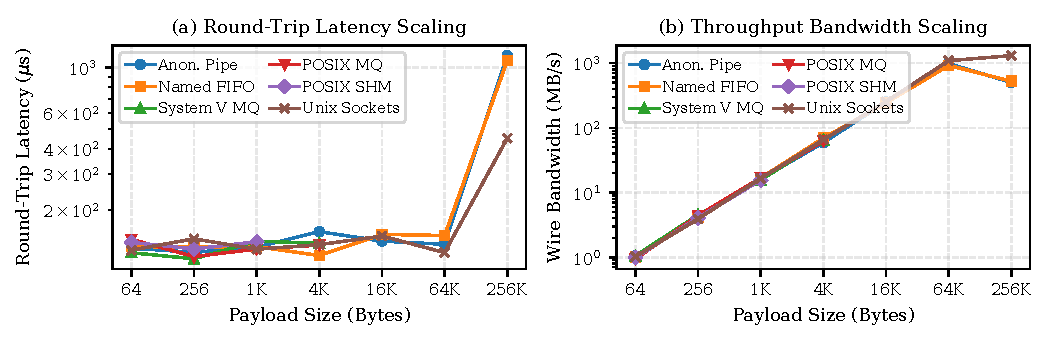
\includegraphics[height=4.2cm]{figures/latency_throughput_combined.pdf}
\caption{Empirical Performance Scaling across Classical Linux IPC Mechanisms on Fedora 45 Linux: (a) Mean Round-Trip Latency ($\mu\text{s}$) vs. Payload Size (log-log scale), and (b) Wire Data Bandwidth (MB/s) vs. Payload Size (log-log scale).}
\label{fig:latency_throughput}
\end{figure*}